\newpage

\section[Программная реализация]{\large \centering Программная реализация}
\hspace{\parindent} Разработанный алгоритм реализован на языке программирования C++ без использования сторонних библиотек и может быть использован на всех основных операционных системах: Windows, Linux, Mac OS. Для удобства использования основного приложения был создан веб-интерфейс, позволяющий осуществлять взаимодействие с программой через графическую оболочку. Поскольку задача множественного выравнивания может требовать существенных вычислительных ресурсов, практично решать ее, используя мощную вычислительную платформу, а взаимодействие с ней осуществлять через веб-интерфейс. Кроме того, для возможности внедрения функций построения парного и множественного выравниваний в другие программы они были реализованы в виде статических библиотек.

\subsection[Структуры данных]{\large Структуры данных}
\hspace{\parindent} В данном разделе описаны используемые в программе структуры данных для хранения и обработки кодирующих последовательностей ДНК. Всего разработано и реализовано три объекта: структура $BioSeq$, описывающая биологические последовательности, класс построения парного выравнивания $PairwiseAlign$ и структура $Profile$ для работы с набором последовательностей. Все они входят в состав собранных статических библиотек и могут быть внедрены в другие проекты.

\subsubsection[Представление биологических последовательностей]{\large Представление биологических последовательностей}
\hspace{\parindent} Для представления биологических последовательностей используется структура $BioSeq$ (листинг~\ref{lst:BioSeq}) с двумя строковыми полями:
\begin{itemize}
	\item $name$ --- идентификатор последовательности
	\item $nt\_seq$ --- последовательность нуклеотидов
\end{itemize}

Ради удобства использования структуры $BioSeq$ был определен оператор индексирования [ ] и функция $Length$, возвращающая текущую длину последовательности. Чтобы иметь связь нуклеотидного и аминокислотного уровней, реализованы методы, позволяющие получить как трансляцию всей строки по первой рамке считывания $std::string$ $GetAAseq()$ $const$, так и конкретного триплета, начинающегося с $i$-го индекса $char$ $TranslateNTtoAA(int$ $i)$ $const$. Также необходимо иметь возможность вставлять разрывы в последовательность, для чего были добавлены методы $InsertGap(int$ $pos)$ и $InsertGap(int$ $pos,$ $int$ $count)$, добавляющие $1$ или $count$ разрывов по индексу $pos$. Печать реализована через перегруженную операцию $<<$. Независимый вывод результатов работы программы как на нуклеотидном, так и на аминокислотном уровнях, осуществляется с помощью методы $void$ $PrintNT(std::ostream\&$ $out)$ и $void$ $PrintAA(std::ostream\&$ $out)$, которые отправляют результат выравнивания на обоих уровнях в указанный поток $out$.
\begin{algorithm}
	\caption{Структура представления биологических последовательностей BioSeq} \label{lst:BioSeq}
	\begin{lstlisting}
struct BioSeq {
  std::string name;
  std::string nt_seq;
  // constructor
  BioSeq(std::string n, std::string s): name(n), nt_seq(s) 
  { } 
  // destructor
  ~BioSeq() { }
  // accessors
  int Length() { return nt_seq.length(); }
  char operator [] (int index) { return nt_seq[index]; }
  void InsertGap(int pos, int count);
  void InsertGap(int pos);
  // translater
  std::string GetAAseq() const;
  char TranslateNTtoAA(int i) const;
  // printer
  void PrintAA(std::ostream& out);
  void PrintNT(std::ostream& out);
  friend std::ostream& operator << (std::ostream& stream,
                                    const BioSeq& data);
};
	\end{lstlisting}
\end{algorithm}

\subsubsection[Класс построения парного выравнивания]{\large Класс построения парного выравнивания}
\hspace{\parindent} Вычисление оптимального выравнивания двух последовательностей реализовано в виде класса $PairwiseAlign$ (листинг~\ref{lst:PairwiseAligner}). Таким образом, в одном объекте собираются и данные, и методы их обработки, что упрощает экспорт алгоритма парного выравнивания в другой проект.\\
\indent Работа с классом подразумевает его использование для повторного решения задачи построения парного выравнивания на различных входных данных. Поэтому класс не содержит полей с исходными последовательностями, в нем хранятся только структуры для построения решения и параметры выравнивания, в частности, штрафы за разрывы, смещение рамки, появление преждевременного стоп-кодона, а также матрицы замен нуклеотидов и аминокислот. Входные данные передаются через метод $Align(const$ $BioSeq*$ $seq1,$ $const$ $BioSeq*$ $seq2)$, реализующий алгоритм парного выравнивания (\ref{PairwiseAlign}). Для увеличения производительности программы вместо использования рекурсивной функции $CalcAlign$ (листинг~\ref{lst:pairwise}) таблицы оптимальных ходов заполняются как в классическом алгоритме Нидлмана-Вунша.\\
\indent Для хранения матриц замен используются два массива: $nt\_score\_matrix$ (нуклеотиды) и $aa\_score\_matrix$ (аминокислоты), размерностью $128\cdot 128$ элементов, поскольку символы строк представлены одним байтом, принимающим значения от 0 до 127 (рисунок~\ref{ris:memory}).
\begin{figure}[H]
	\center{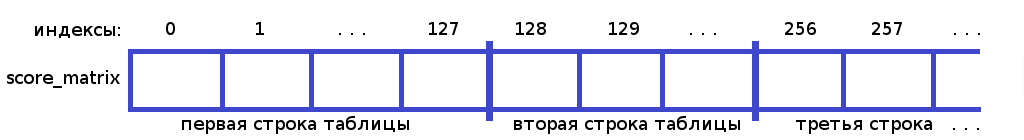
\includegraphics[width=0.95\linewidth]{memory.png}}
	\caption{Представление матрицы замен в памяти компьютера}
	\label{ris:memory}
\end{figure}
\indent Используя данный подход, на вход программе выравнивания можно подавать последовательности с символами из произвольного алфавита. Для этого необходимо лишь определить соответствующие матрицы замен и предоставить функцию для трансляции кодонов. Адресация по массиву определена следующим образом:
\begin{equation*}
nt\_score\_matrix[(unsigned\hspace{0.2cm} char)'A'*128+(unsigned\hspace{0.2cm} char)'C']
\end{equation*}
Пример отражает цену за сопоставление аденина ($A$) и цитозина ($C$). В общем случае вместо конкретных нуклеотидов в формулу подставляются $i$-ый и $j$-ый символы строк: $seq1[i]$, $seq2[j]$.

\begin{algorithm}[H]
	\caption{Класс построения оптимального выравнивания двух последовательностей} \label{lst:PairwiseAligner}
	\begin{lstlisting}
class PairwiseAlign {
private:
  int gap_open, gap_extension, gap_frame, stop_cost;
  int nt_score_matrix[128*128];
  int aa_score_matrix[128*128];
  int seq1_length, seq2_length; 
  int matrix_size = 0;
  int* F = NULL; // score matrix
  int* W = NULL; // way matrix
  void NewScoreMatrix(const char* file_name, 
  			int* score_matrix);

public:
  PairwiseAlign(const char* nt_score_matrix, 
      const char* aa_score_matrix, int stop_cost, 
      int gap_open, int gap_extension, int frame_gap);
  ~PairwiseAlign() { 
  	if (F) delete[] F; 
  	if (W) delete[] W; 
  }
  
  // calc align 
  int Align(const BioSeq* seq1, const BioSeq* seq2);
  std::pair<std::string, std::string> GetAlign();
  
  // change substitution matrices
  void ChangeNTscoreMatrix(const char* file_name) {
    return NewScoreMatrix(file_name, nt_score_matrix);
  }
  void ChangeAAscoreMatrix(const char* file_name) {
    return NewScoreMatrix(file_name, aa_score_matrix);
  }
  
  // accessors
  int GetGapOpen() { return gap_open; } 
  	\end{lstlisting}
\end{algorithm}

\begin{algorithm}
	\begin{lstlisting}
  int GetGapExtension() { return gap_extension; } 
  int GetGapFrame() { return gap_frame; } 
  int GetStopCost() { return stop_cost; } 
};
	\end{lstlisting}
\end{algorithm}

\subsubsection[Профили]{\large Профили}
\hspace{\parindent} Выравненные строки сохраняются в структуру $Profile$ (листинг~\ref{lst:ProfileStruct}). Для экономии памяти и времени в профили заносятся не копии последовательностей, а только указатели на них. Функция объединения записана в виде перегруженной операции $+$. Кроме этого, профили имеют методы для вычисления оценки за сопоставление двух столбцов нуклеотидов и аминокислот. Так же, как и для структуры $BioSeq$, реализована возможность вставки разрывов по указанному индексу заданной длины. Дополнительно у профилей имеется массив $frequency$, содержащий частоты распределения нуклеотидов и аминокислот в конкретной позиции. Для его заполнения реализованы методы $CalcFrequenciesNT$ и $CalcFrequenciesAA$.\\
\begin{algorithm}
	\caption{Структура профилей} \label{lst:ProfileStruct}
	\begin{lstlisting}
struct Profile {
  Profile();
  ~Profile();
  // data
  std::vector<BioSeq*> sequences;
  int frequency[128];
  // alignment of profiles and sequence
  Profile& operator + (Profile& another);
  Profile& operator + (BioSeq* sequence);
  // get score in column
  float ColumnNTscore(BioSeq* seq, int index1, 
  				   int index2);
  float ColumnAAscore(BioSeq* seq, int index1, 
  				   int index2);
  float ColumnNTscore(Profile& another, int index1, 
  					int index2);
  float ColumnAAscore(Profile& another, int index1, 
   					int index2);
  	\end{lstlisting}
\end{algorithm}

\begin{algorithm}
	\begin{lstlisting}
  // fill an array of frequency
  void CalcFrequenciesNT(int position);
  void CalcFrequenciesAA(int position);
  // insert gaps in sequences
  void InsertGap(int pos, int count);
  void InsertGap(int pos);  
};
	\end{lstlisting}
	
\end{algorithm}

\indent Предложенное нами программное решение обеспечивает защиту последовательностей, входящих в состав профиля, от изменения или удаления до конца построения выравнивания. В противном случае возможно было бы появление ошибок выполнения или ухудшение качества результата. При экспорте разработчик должен уделить внимание этому аспекту.

\subsection[Общая схема работы]{\large Общая схема работы}
\hspace{\parindent} На рисунке~\ref{ris:scheme} изображена блок-схема работы программы. Основные этапы реализованы в виде отдельных, независимых друг от друга блоков, что дает возможность модифицировать их или заменить новыми. 
\begin{figure}[H]
	\center{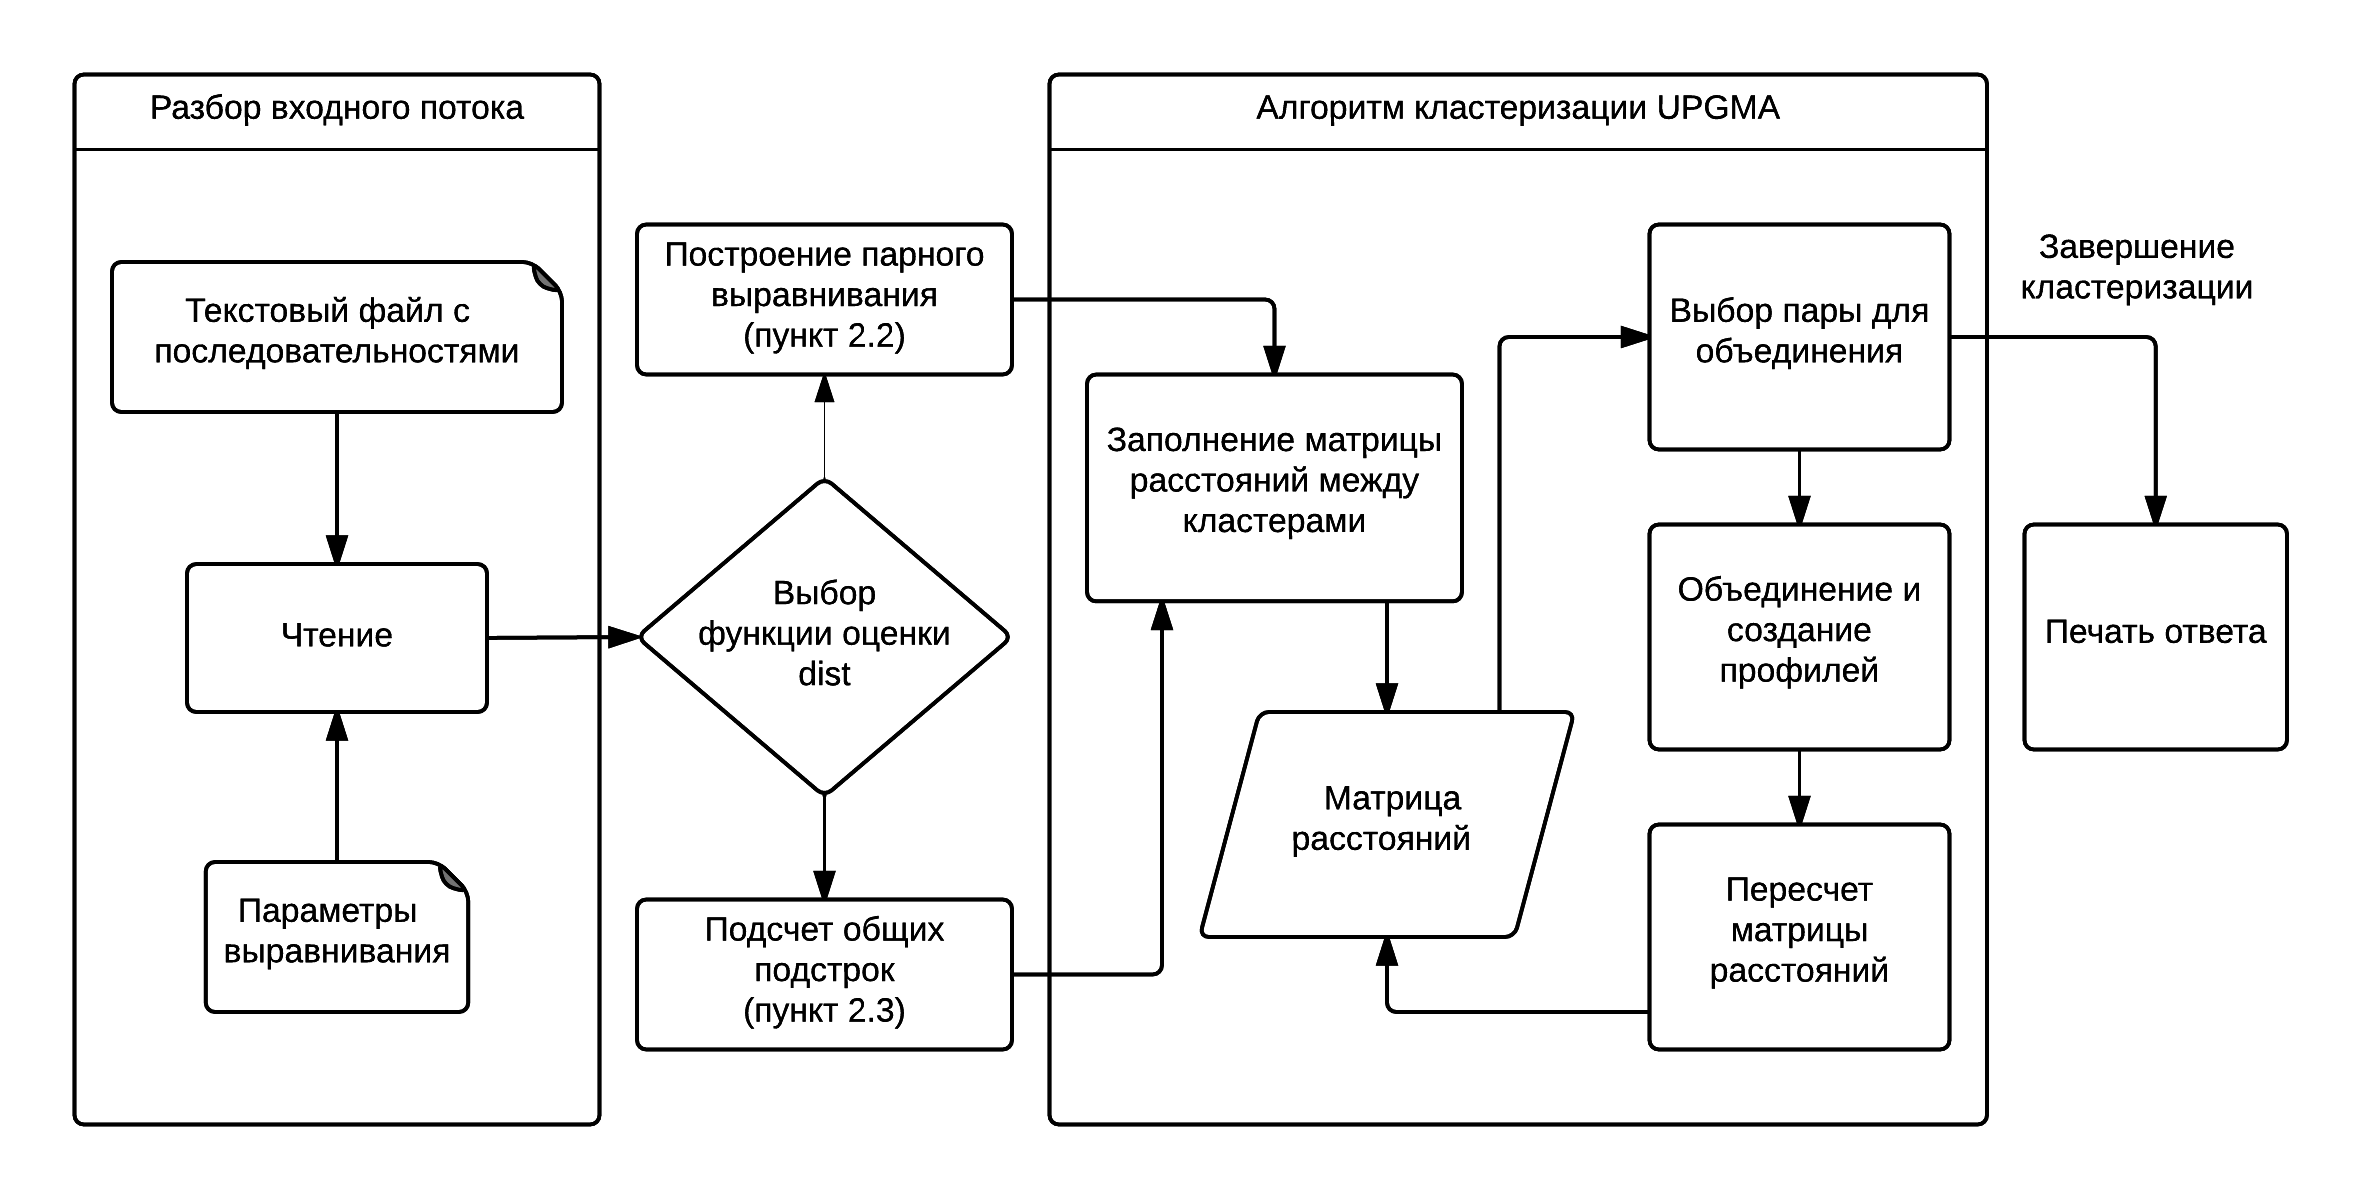
\includegraphics[width=1\linewidth]{block-scheme.png}}
	\caption{Блок-схема работы программы}
	\label{ris:scheme}
\end{figure}

\subsubsection[Чтение входных данных]{\large Чтение входных данных}
\hspace{\parindent} На вход программе подается текстовый файл с последовательностями в формате FASTA~\cite{FASTAformat}. Строка, начинающаяся с символа '>', называется строкой описания. Она содержит имя последовательности и некоторую дополнительную информацию, предназначенную для идентификации. Другие строки, начинающиеся с символа ';', являются комментариями и игнорируются. За строкой описания следует код последовательности. При кодировании нуклеотидов буквами A, C, G и T кодируют, соответственно, аденин, цитозин, гуанин и тимин. На рисунке~\ref{ris:FASTAexample} представлен пример тестового файла в формате FASTA.
\begin{figure}[H]
	\center{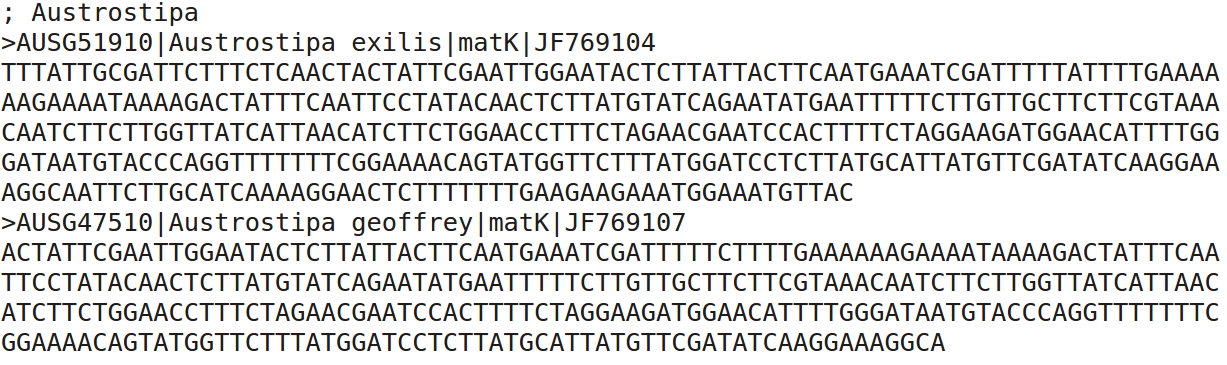
\includegraphics[width=1.\linewidth]{FASTAexample.png}}
	\caption{Пример файла в формате FASTA}
	\label{ris:FASTAexample}
\end{figure}

Программа может использовать для вычисления очков за сопоставление нуклеотидов и аминокислот пользовательские матрицы замен. Их необходимо представить в таком же формате, как и на рисунке~\ref{ris:BLOSUM62}.
Строки, начинающиеся с символа $\#$, являются комментариями и игнорируются, а при задании таблицы первые строка и столбец определяют символы сопоставления. Количество пробелов может быть любым.

\begin{figure}[h]
	\center{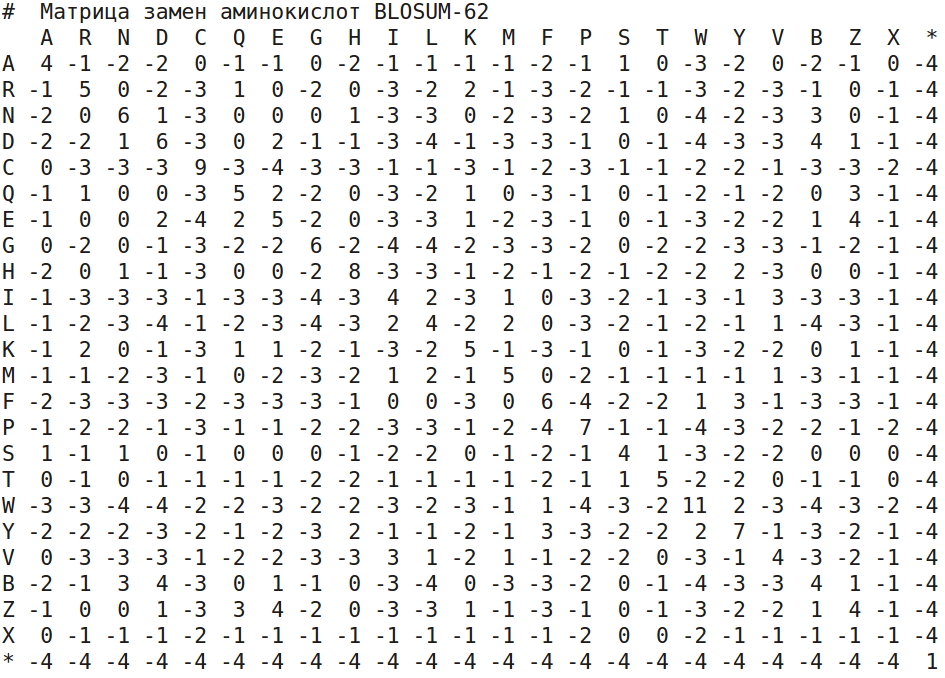
\includegraphics[width=0.9\linewidth]{BLOSUM62.png}}
	\caption{Пример файла с матрицей замен}
	\label{ris:BLOSUM62}
\end{figure}

\subsubsection[Определение порядка выравниваний]{\large Определение порядка выравниваний}
\hspace{\parindent} Алгоритм кластеризации реализован в виде процедуры, принимающей на вход массив последовательностей и функцию оценки расстояния между ними --- $dist$. Пользователь может выбрать, что использовать в качестве оценки $dist$: метод построения парного выравнивания $Align$ из класса $PairwiseAlign$ или подсчет количества одинаковых подпоследовательностей заданной длины $k$. Существует возможность использования своей собственной функции расстояния. Для этого ее необходимо определить как $std::function<int$~$(BioSeq*$, $BioSeq*)>$. \\
\indent На каждом шаге алгоритма не происходит выделение новой памяти для перехода от старой таблицы размерности $n$ к новой $n-1$. Используется дополнительный массив, в котором хранится информация о том, какие строки и столбцы матрицы более неактивны и пропускаются при переборе. На рисунке~\ref{ris:UPGMA-2} показан пример пересчета таблицы расстояний с указанием неактивных строк и  обновляемых на каждом этапе элементов. 

\begin{figure}[h]
	\center{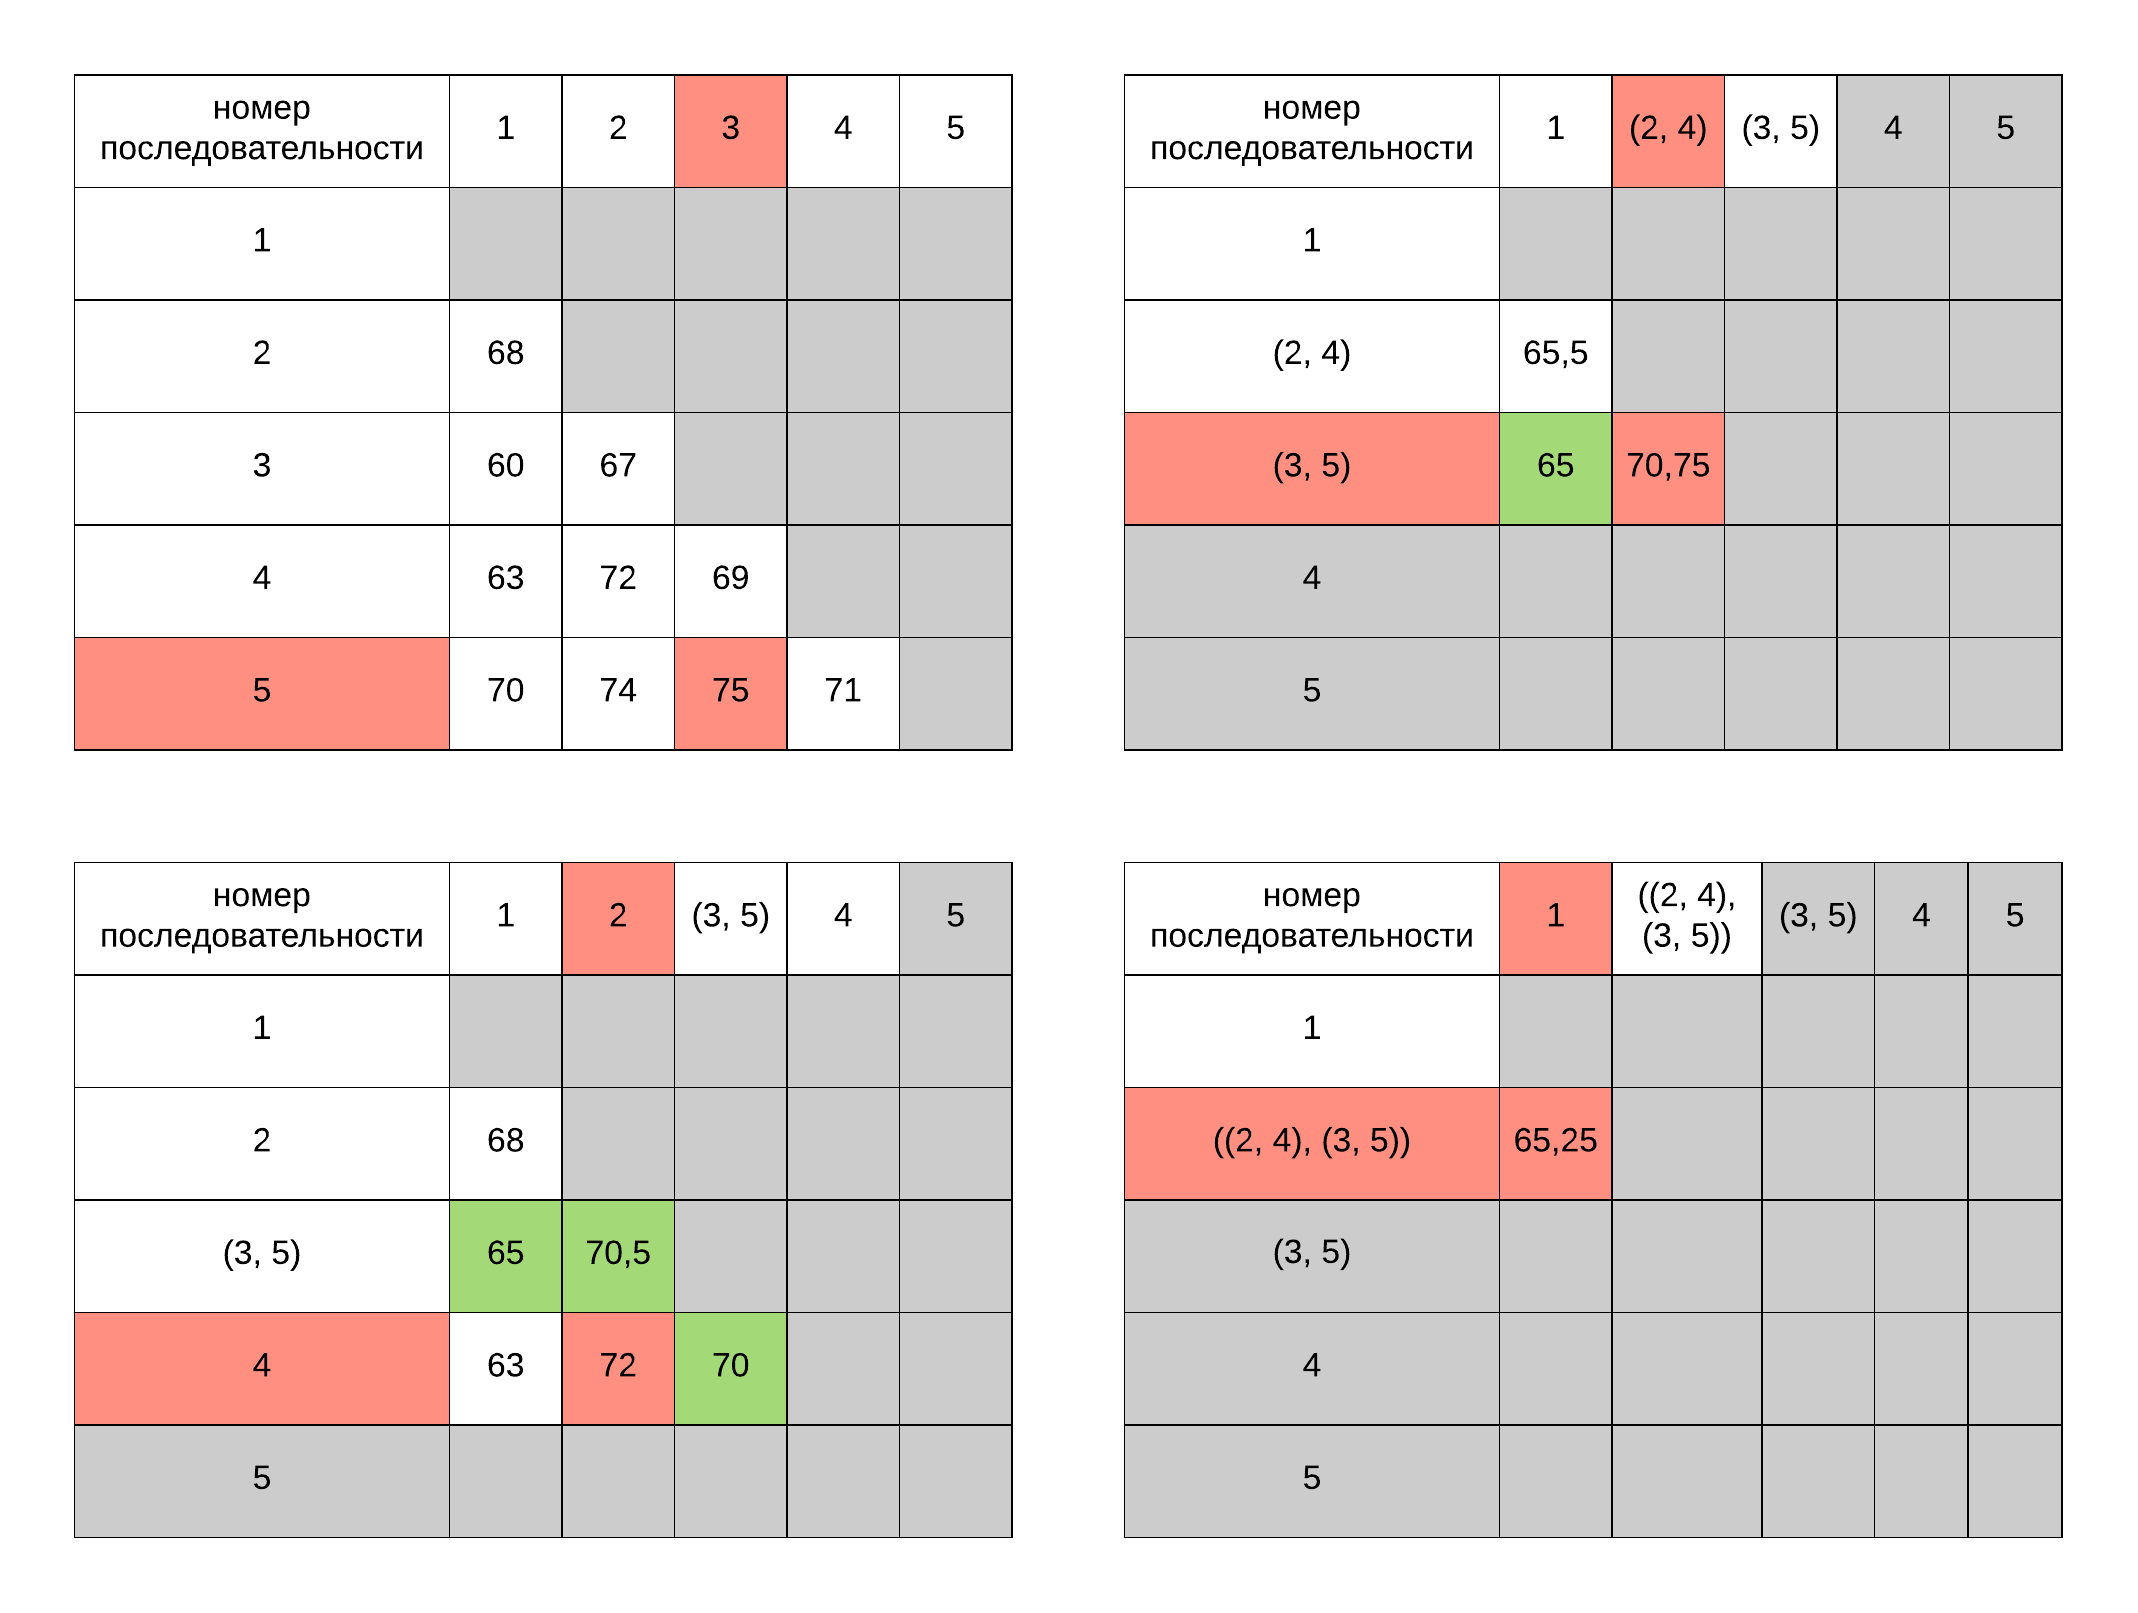
\includegraphics[width=0.9\linewidth]{UPGMA-2.png}}
	\caption{Пересчет матрицы расстояний. Красным отмечены элементы для объединения, зеленым --- обновленные значения, серым --- неактивные ячейки.}
	\label{ris:UPGMA-2}
\end{figure}

Такой подход позволяет экономить время выполнения программы за счет избавления от операций выделения новой таблице на каждом шаге алгоритма кластеризации. Кроме того, алгоритм экономно использует память компьютера.

\subsubsection[Объединение профилей]{\large Объединение профилей}
\hspace{\parindent} При объединении профилей $P_1$ и $P_2$ происходит рассчет оптимального выравнивания с заполнением матрицы размерности $len(P_1) \cdot len(P_2)$. Для того чтобы сократить количество выделений памяти, было решено сохранять заполненную таблицу после операции объединения. Таким образом, новая память будет выделена только в том случае, если текущая размерность матрицы, оставшейся с предыдущей итерации, не удовлетворяет размерности очередной пары профилей. На листинге~\ref{lst:ProfilePlus} представлен алгоритм объединения.

\begin{algorithm}[H]
	\caption{Алгоритм объединения профилей} \label{lst:ProfilePlus}
	\begin{algorithmic}
		\State $F \gets [$ $]$ \Comment{Матрица оптимальных ходов}
		\Procedure{$ProfileMerge$}{$P_1, P_2$}
		\State \Comment{Проверка размерности матрицы}
		\If{$size(F)$ $<$ $len(P_1)$ OR $size(F)$ $<$ $len(P_2)$} 
			\State $new\_size \gets max(len(P_1), len(P_2))$
			\State $F \gets [new\_size \times new\_size]$ \Comment{Выделение новой памяти}
		\EndIf
		\algstore{bkbreak}
	\end{algorithmic}
\end{algorithm}

\begin{algorithm}
	\begin{algorithmic}
		\algrestore{bkbreak}
		\For{$i = 1 \cdots len(P_1)$} \Comment{Цикл заполнения таблицы переходов}
			\For{$j = 1 \cdots len(P_2)$}
				  \State \Comment{Позиция текущей ячейки --- $i$, $j$}
			      \State \text{Рассчет оптимального перехода,} 
		        \State \text{перебор 25 возможных вариантов}
		    \EndFor
        \EndFor
		\While{ответ не построен} \Comment{Цикл построения ответа}
			\State \text{Определить переход на $i$-ом шаге}
			\State \text{Изменить последовательности в профилях}
			\State \text{Перейти по таблице на следующую ячейку}
        \EndWhile		
		\EndProcedure
		\State $P_1 \gets$ добавить все последовательности из $P_2$
		\State \textbf{return} $P_1$
	\end{algorithmic}
\end{algorithm}

\subsection[Руководство пользователя]{\large Руководство пользователя}
\subsubsection[Опции компиляции]{\large Опции компиляции}
\hspace{\parindent} Ниже приведены команды сборки разработанного приложения для компилятора gcc~\cite{GCC} версии 4.8.4. Подразумевается, что в директории, где происходит компиляция, находятся только исходные коды описанной программы. При сборке необходимо указать стандарт языка c++11, а также для повышения производительности добавить опцию оптимизации -O3:
\begin{equation*}
\texttt{g++ -std=c++11 -O3 *.c++ -o multy}
\end{equation*}
\indent Для получения версии с печатью отладочной информации в процессе построения выравнивания (вывод матрицы оптимальных ходов, текущих результатов объединения профилей и таблицы расстояний на каждом шаге кластеризации) нужно воспользоваться следующей командой:
\begin{equation*}
\texttt{g++ -std=c++11 -DDEBUG *.c++ -o multy}
\end{equation*}
\indent Использование такой сборки предполагает поиск и устранение ошибок, возникающих в процессе выравнивания. В таком случае к команде компиляции добавляют опции -g и -O0, отвечающие за предоставление отладочных символов в исполняемом файле и отсутствие оптимизации. После устранения всех ошибок и переходу к этапу тестирования можно воспользоваться сборкой, предоставляющей информацию о времени выполнения различных этапов алгоритма:
\begin{equation*}
\texttt{g++ -std=c++11 -DTIME -O3 *.c++ -o multy}
\end{equation*}
\indent Также для удобства использования был написан Makefile --- набор инструкций для программы make~\cite{MAKE}, благодаря которому сборка всего решения производится одной командой: make, или make DEBUG --- для получения версии с отладочной информацией.\\
\indent Используемая в предыдущих командах компиляции опция -o определяет имя полученной программы. Для конкретизации обозначения разработанного приложения множественного выравнивания было выбрано название multy (от английского multiple --- множественный).

\subsubsection[Параметры запуска]{\large Параметры запуска}
\hspace{\parindent}
Работа с программой представлена в двух вариантах: через консольное приложение или веб-интерфейс. В таблице~\ref{tabular:options} перечислены все возможные опции для запуска исполняемого файла.
\begin{table}[H]
\small
\caption{Опции программы}
\label{tabular:options}
\begin{center}
\begin{tabular}{|p{2.4cm}|p{3.5cm}|p{5.cm}|p{4.4cm}|}
\hline
Сокращенные опции& Полные опции& Значение& Комментарий\\
\hline
$-h$& $--help$& без аргумента& вывод справочной информации\\
\hline
$-i$& $--input$& путь к файл с последовательностями & файл должен быть представлен в формате FASTA\\
\hline
$-n$& $--NT\_subst$& путь к файлу с матрицей замен для нуклеотидов & по умолчанию: +4 за сопоставление одинаковых нуклеотидов и -5 в противном случае\\
\hline
$-a$& $--AA\_subst$& путь к файлу с матрицей замен для аминокислот& по умолчанию используется матрица замен BLOSUM62~\cite{BLOSUM62}\\
\hline
\end{tabular}
\end{center}
\end{table}

\begin{table}[H]
\small
\begin{center}
\begin{tabular}{|p{2.4cm}|p{3.5cm}|p{5.cm}|p{4.4cm}|}
\hline
Сокращенные опции& Полные опции& Значение& Комментарий\\
\hline
$-g$& $--gap\_open$& штраф за открытие разрыва& значение по умолчанию: -10\\
\hline
$-e$ & $--gap\_extension$& штраф за продолжение разрыва& значение по умолчанию: -3\\
\hline
$-f$& $--gap\_frame$& штраф за разрыв рамки& значение по умолчанию: -15\\
\hline
$-s$& $--stop\_cost$& штраф за преждевременное появление стоп-кодона& значение по умолчанию: -50\\
\hline
$-d$& $--dimension$& начальная размерность матрицы для объединения профилей& значение по умолчанию: 1024$\times$1024\\
\hline
$-k$& $--k-mers$& необязательный числовой аргумент $k$& использовать в качестве функции $dist$ алгоритм подсчета общих подстрок длины $k$; значение по умолчанию для $k$: 10 \\
\hline
$-p$& $--pairwise$& без аргумента& использовать в качестве функции $dist$ алгоритм построения парного выравнивания\\
\hline
\end{tabular}
\end{center}
\end{table}

При запуске приложения без указания входного файла или с использованием неверных опций будет выдано соответствующее сообщение об ошибке. В случае корректного задания входных параметров произойдет чтение и разбор указанного набора последовательностей, после чего будет напечатана вся информация по заданной задаче выравнивания: количество полученных последовательностей, матрицы замен и параметры штрафов (листинг~\ref{lst:multyRun}).

\begin{algorithm}[H]
	\caption{Примеры запуска программы} \label{lst:multyRun}
	\begin{lstlisting}
$ ./multy -s -40 -f 20
nothing to align

$ ./multy -i ENAM_genes.fasta --AA_substitution BLOSUM60
./multy: unrecognized option '--AA_substitution'

$ ./multy -i ENAM_genes.fasta 
Reading sequences...
7 sequences were obtained
Input parameters:
NT substitution matrix	NUC-45
	\end{lstlisting}
\end{algorithm}

\begin{algorithm}
	\begin{lstlisting}
AA substitution matrix	BLOSUM62
Gap open cost		-10
Gap extension cost	-3
Gap frame cost		-15
Stop codon cost		-50

$ ./multy -i ENAM_genes.fasta -s -40 --AA_subst BLOSUM60
Reading sequences...
7 sequences were obtained
Input parameters:
NT substitution matrix	NUC-45
AA substitution matrix	BLOSUM60
Gap open cost		-10
Gap extension cost	-3
Gap frame cost		-15
Stop codon cost		-40
	\end{lstlisting}
\end{algorithm}

На рисунке~\ref{ris:webka} изображен графический интерфейс для работы с программой. Форму можно условно разделить на две части: поле ввода данных и область задания параметров выравнивания. 

\begin{figure}[H]
	\center{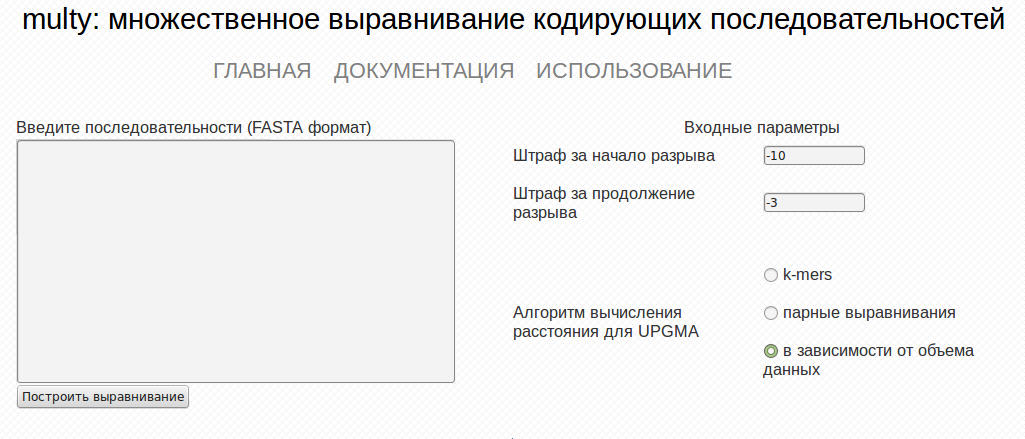
\includegraphics[width=1.\linewidth]{web.png}}
	\caption{Графический интерфейс для построения выравнивания}
	\label{ris:webka}
\end{figure}

После ввода последовательностей и указания необходимых параметров необходимо нажать на кнопку <<построить выравнивание>>. По окончании работы будет загружена страница с результатами выравнивания (рисунок~\ref{ris:webkares}).

\begin{figure}[h]
	\center{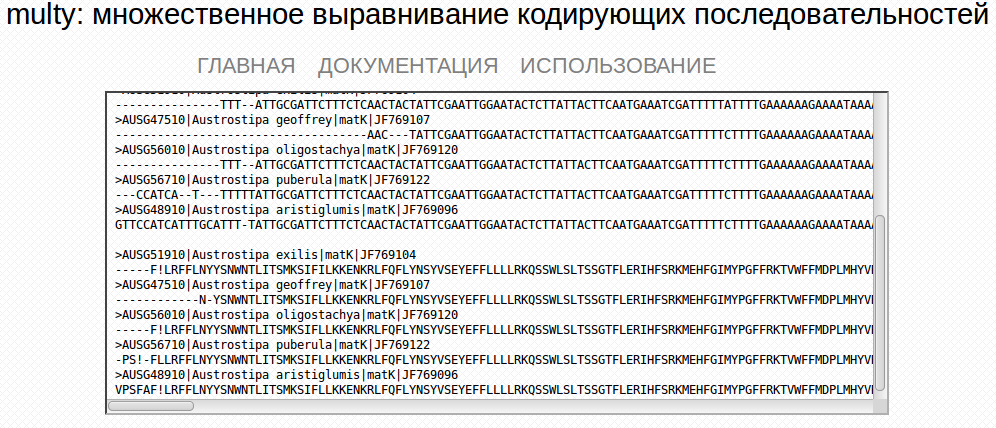
\includegraphics[width=1.0\linewidth]{webres.png}}
	\caption{Форма с результатами выравнивания}
	\label{ris:webkares}
\end{figure}

\subsubsection[Использование собранных библиотек]{\large Использование собранных библиотек}
\hspace{\parindent} В данном разделе описана работа с собранными статическими библиотеками построения парного ($libpairwise.a$) и множественного ($libmulty.a$) выравниваний. В таблице~\ref{tabular:staticlibs} представлена информация о входящих в состав библиотек структур данных и функциях.

\begin{table}[h]
\caption{Содержание статических библиотек}
\centering
\begin{tabular}{|l|l|}
\hline
Библиотека & Содержание \\ \hline
\multicolumn{ 1}{|c|}{libpairwise.a} & структура BioSeq \\ \cline{ 2- 2}
\multicolumn{ 1}{|l|}{} & класс PairwiseAlign \\ \cline{ 2- 2}
\multicolumn{ 1}{|l|}{} & функция чтения файла в формате FASTA \\ \hline
\multicolumn{ 1}{|c|}{libmulty.a} & структура BioSeq \\ \cline{ 2- 2}
\multicolumn{ 1}{|l|}{} & структура Profile \\ \cline{ 2- 2}
\multicolumn{ 1}{|l|}{} & функция чтения файла в формате FASTA \\ \cline{ 2- 2}
\multicolumn{ 1}{|l|}{} & функция кластеризации по алгоритму UPGMA \\ \hline
\end{tabular}
\label{tabular:staticlibs}
\end{table}

В проект необходимо подключить заголовочные файлы с используемыми структурами и функциями (листинг~\ref{lst:LibHeader}). Функция $ReadFastaFile$ осуществляет чтение последовательностей из указанного файла $input\_fasta$ и сохраняет их в массив $buf$. В случае возникновения ошибки она вернет значение 1, иначе --- 0. Алгоритм кластеризации реализован через функцию $UPGMA$, принимающей на вход набор последовательностей $sequences$, функцию оценки расстояния $dist$ и параметры выравнивания для объединения кластеров (названия параметров соответствуют именам коротких опций программы). Вызов данной функции приведет к изменению данных в массиве $sequences$, он будет содержать результаты выравнивания.

\begin{algorithm}
	\caption{Прототипы библиотечных функций} \label{lst:LibHeader}
	\begin{lstlisting}
int ReadFastaFile(char* input_fasta, 
			std::vector<BioSeq*>& buf);
			
// distance function type
typedef std::function<int (BioSeq* seq1, 
			BioSeq* seq2)> func;
			
// UPGMA function change input sequences!
void UPGMA(std::vector<BioSeq*>& sequences, func dist, 
	// input parameters
	int g, int e, int f, int s, const int* n, 
	const int* a);
	\end{lstlisting}
\end{algorithm}

При сборке приложения c импортированными методами и структурами построения выравниваний необходимо указать компилятору используемую библиотеку. Ниже представлен пример компиляция новой программы из исходного файла $new\_program.c++$ с библиотекой $libmulty.a$: 
\begin{equation*}
\texttt{g++ -std=c++11 -L./ -lmulty new\_program.c++ }
\end{equation*}